\chapter{Aspectos Conceituais} \label{cap:conceitos}

Para realizar a ambição de desenvolver um \textit{dongle} seguro, é necessário entender, primeiramente, o contexto no qual este dispositivo atuará; as especificações às quais ele deve sujeitar-se; e as possibilidades que fornecerá ao seu usuário.

A coleta dos dados é possibilitada pela existência da rede CAN, uma rede veicular que toma a forma de um barramento de dois fios, pelos quais trafegam as mensagens trocadas entre as ECUs. Ela será devidamente detalhada na seção \autoref{sec:CAN}; presentemente basta identificar que a rede CAN define somente as camadas física e de dados. Um protocolo de alto nível é necessário para gerenciar a comunicação e padronizar as mensagens.

Neste contexto, o protocolo OBD-II é adotado. Ele especifica, entre outros, a forma da comunicação, que ocorre no modelo requisição-resposta, e o formato das mensagens e dos dados nelas contidos. Também será oportunamente detalhado na \autoref{sec:OBD}. 

Nota-se que um dispositivo que deseje participar de comunicação OBD-II com um automóvel deve conectar-se à rede CAN do carro e saber modular suas mensagens nos dois fios que compõem o barramento, bem como identificar neles a resposta à sua requisição. Este é um processo trabalhoso e convidativo à abstração. Isto levou ao surgimento do ELM327, um \textit{dongle} que se conecta à porta OBD-II e fornece uma interface serial para um cliente, comumente um PC, que pode enviar e receber mensagens ASCII, as quais serão traduzidas para o formato das mensagens OBD-II. 

A implementação do \textit{dongle} proposto tomará, como modelo, o ELM327, cuja inspiração materializar-se-á em uma camada responsável por receber e enviar caracteres, processar comandos AT de autoconfiguração, e filtrar mensagens. Os pontos relevantes do ELM327 serão detalhados na seção \autoref{sec:ELM}.

O ESP32 é um microcontrolador (...) e será utilizado para implementação do \textit{dongle} proposto. Para possibilitar a integração do \textit{dongle} com um aplicativo móvel, optou-se pela utilização do Bluetooth Low Energy. Para a programação do ESP32, optou-se pela utilização do PlatformIO e freetros  

O microcontrolador escolhido para a implementação do \textit{dongle} proposto 
é o ESP32, um sistema em chip (SoC) que integra, entre outros periféricos, 
um controlador CAN e um módulo de comunicação Bluetooth, tornando-o adequado 
para os requisitos do projeto. Para possibilitar a integração do 
\textit{dongle} com um aplicativo móvel, optou-se pela utilização do 
Bluetooth Low Energy. Já para a programação do ESP32, optou-se pela 
utilização do FreeRTOS, um sistema operacional de tempo real que permitirá 
a organização do firmware em tarefas concorrentes, e do PlatformIO, ambiente 
de desenvolvimento que facilita o gerenciamento de dependências e a 
compilação do projeto.

// ADICIONAR PEQUENO PARAGRAFO SOBRE DART E APP

Com isso, estão dispostas todas as camadas que compõem o cenário do projeto, e cujo entendimento será indispensável para sua implementação. As seções seguintes, portanto, dedicar-se-ão ao detalhamento de cada uma delas.

\begin{figure}[H]
    \centering
    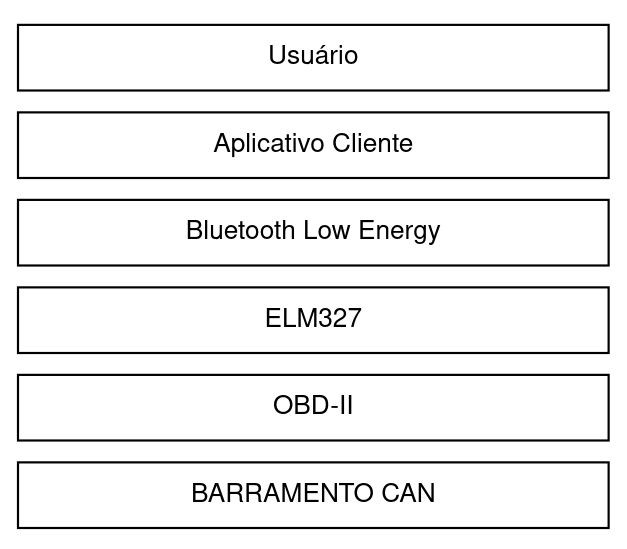
\includegraphics[width=0.6\textwidth]{assets/cap2-conceitos/camadas.png}
    \caption{Camadas que compõem o cenário do projeto}
    \label{fig:camadas}
    \fonte{Os autores (2026)}
\end{figure}


\section{Rede CAN} \label{sec:CAN}

A rede CAN foi especificada pela Bosch na década de 80 (TODO: MELHORAR), e é utilizada em veículos para permitir a comunicação confiável entre as suas unidades controladoras eletrônicas (ECUs). Ela especifica a camada física e a camada de dados.

DIAGRAMA DO BARRAMENTO CAN

EXPLICAÇÃO PREOCUPAÇÕES CAN - RELIABILITY; DETECÇÃO DE ERRO; DETECÇÃO DE COLLISÃO; ARBITRAGEM NÃO DESTRUTIVA 

EXPLICAÇÃO CONTROLADOR CAN - ADESÃO AO  PROTOCOLO CAN; ENCODING; ERROR DETECTION; ARBITRAGEM; SELF-DISCONNECT AO IDENTIFICAR MAU FUNCIONAMENTO PARA EVITAR ATRAPALHAR O BARRAMENTO; ETC

EXPLICAÇÃO TRANSCEIVER CAN - CONVERTE SINAIS LÓGICOS ÀS TENSÕES FÍSICAS NAS DUAS LINHAS DO BARRAMENTO

EXPLICAÇÃO FORMATOS DE UMA MENSAGEM CAN; DESTAQUE AO CAMPO "DATA", QUE CONTERÁ AS MENSAGENS OBD-II

\section{Protocolo OBD-II} \label{sec:OBD}

OBD-II REQUER QUE A CAMADA FÍSICA SUBJACENTE SEJA CAN; PODE SER 250 Kbits OU 500 kbits; O CAMPO CAN ID PODE TER 11 bits OU 29 bits; CAN IDS ESPECÍFICOS SÃO UTILIZADOS PARA REQUISIÇÕES E RESPOSTAS OBD; AS RESPOSTAS PODEM CABER EM UMA ÚNICA MENSAGEM (SINGLE FRAME) OU SERÃO DIVIDIDAS EM MÚLTIPLAS (MULTI-FRAME; ISO TP) 

OBD-II DEFINE CONECTOR; PINOS; EXPLICITAR QUE UM DOS PINOS É 12V, QUE É DA BATERIA DO CARRO

DIAGRAMA DOS CAMPOS DE UMA MENSAGEM OBD-II

EXPLICAÇÃO OBD-2 DEFINE SERVIÇOS (MODOS) E PIDS; EXPLICAÇÃO DOS PIDS PADRONIZADOS; PIDS DE DISCOVERY; ETC

TABELA COM PIDS PADRONIZADOS 

EXEMPLO DE UM CICLO REQUISIÇÃO-RESPOSTA OBD-II

EXPLICAÇÃO QUE UMA REQ PODE SER ATENDIDA POR MAIS DE UMA ECU

DIAGRAMA DE EXEMPLO DE UMA COMUNICAÇÃO ATENDIDA POR MAIS DE UMA ECU, COM FIRST FRAME, FLOW CONTROL, CONSECUTIVE FRAME

RESUMO DO QUE PODE SER CONSULTADO VIA OBD-II

\section{ELM327} \label{sec:ELM}

EXPLICAR QUE ELM-327 ORIGINALMENTE POSSIBILITA ASCII, MAS EXPLICITAR QUE SUA PREOCUPAÇÃO RESTRINGE-SE SOMENTE À TRADUÇÃO, CONFORME DOC:

""One must keep in mind that the ELM327 is a protocol interpreter that makes no attempt to assess the OBD messages for validity – it only ensures that hexadecimal digits were received, combined into bytes, then sent out the OBD port, and it does not know if a message sent to the vehicle was in error.""

EXPLICAR QUE PODE RECEBER COMANDOS AT PARA CONFIGURAÇÃO PRÓPRIA; EXEMPLOS DE COMANDOS AT. 

EXEMPLO DE COMUNICAÇÃO: ENVIA UM PID EM ASCII (EX. 010C ), RECEBE DADOS HEXADECIMAIS NA SAÍDA; CONVERTE ELES

COM ISTO DEVERÁ FICAR CLARO A COMUNICAÇÃO PONTA-A-PONTA.


\section{Bluetooth Low-Energy} \label{sec:BLE}

EXPLICAR O QUE É BLUETOOTH LOW ENERGY; DIFERENÇA AO CONVENCIONAL; GATT, SERVER, CLIENT, SERVICES, CHARACTERISTICS, GAP. SERIAL-OVER-BLE. NORDIC UUIDS PARA RX E TX.


\section{FreeRTOS e Arduino}

PARA QUE SERVE O FREERTOS; CONCEITOS BÁSICOS; TASKS; FILAS. 

\section{PlatformIO}

PLATFORMIO; VARIÁVEIS DE AMBIENTE; PERFIS DE COMPILAÇÃO

\section{Ataques}

MODELAGEM DE ATAQUES POSSÍVEIS